\chapter{Project overview}

Snake is a game where the objective is making a line (the snake) grow by eating fruits. The game area is enclosed by a border. The rules are not to hit the border, or the line, itself, because if hit the game is over. This gets increasingly harder, as the line grows in size.

Our game (Snake) is built for the Atmel AVR Mega32 microcontroller. To display the game, we'll use the same type of screen found in the Nokia 3310 and to control the game, we'll use a NES controller.

Thus, we have defined three blocks that outlines our system, as seen in the Block Definition Diagram in Figure~\ref{fig:bdd}. The official responsibilities of the blocks in Figure~\ref{fig:bdd} is as follows:

\begin{itemize}
	\item \textbf{Mega32}: Runs the game, processes input from the controller and draws game on the display.
	\item \textbf{Display}: Displays the game.
	\item \textbf{Controller}: Controls the game.
\end{itemize}

\begin{figure}
\centering
\includegraphics[width=0.7\textwidth, trim={5mm 5mm 5mm 0mm}, clip]{overview/bdd}
\caption{Block Definition Diagram}
\label{fig:bdd}
\end{figure}

\chapter{Architecture}

We have defined three blocks that outlines our system, as seen in the Block Definition Diagram in Figure~\ref{fig:bdd}. The official responsibilities of the blocks in Figure~\ref{fig:bdd} is as follows:

\begin{itemize}
	\item \textbf{Mega32}: Runs the game, processes input from the controller and draws game on the display.
	\item \textbf{Display}: Displays the game.
	\item \textbf{Controller}: Controls the game.
\end{itemize}

\begin{figure}
\centering
\includegraphics[width=0.7\textwidth, trim={5mm 5mm 5mm 0mm}, clip]{architecture/bdd}
\caption{Block Definition Diagram}
\label{fig:bdd}
\end{figure}

We've identified the Display as a PCD8544. We've also found out that the NES controller uses a CD/TC4021 (8-stage static shift register) to store the state of the controller. Therefore, we'll have write at least two drivers for our system: one to interface the display and one to interface the controller.

We have chosen to describe our system using an Internal Block Diagram (IBD) as seen in Figure~\ref{fig:ibd}. The IBD shows the connections between the blocks.

\begin{figure}
\centering
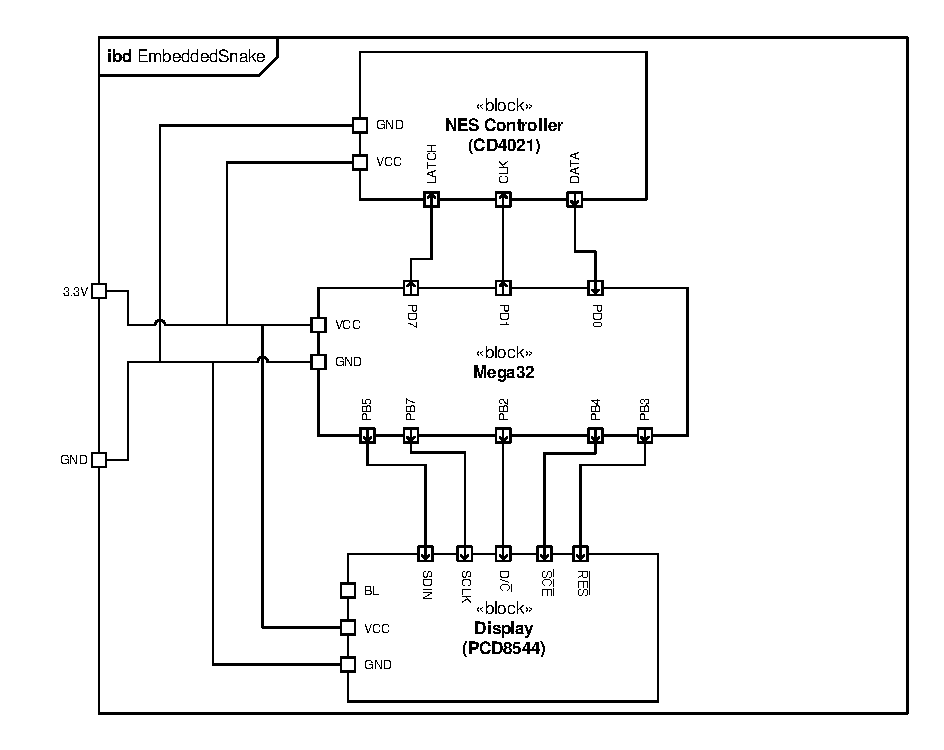
\includegraphics[width=0.8\textwidth, trim={10mm 5mm 5mm 0mm}, clip]{architecture/ibd}
\caption{Internal Block Diagram}
\label{fig:ibd}
\end{figure}

\chapter{Architecture}

We have defined three blocks that outlines our system, as seen in the Block Definition Diagram in Figure~\ref{fig:bdd}. The official responsibilities of the blocks in Figure~\ref{fig:bdd} is as follows:

\begin{itemize}
	\item \textbf{Mega32}: Runs the game, processes input from the controller and draws game on the display.
	\item \textbf{Display}: Displays the game.
	\item \textbf{Controller}: Controls the game.
\end{itemize}

\begin{figure}
\centering
\includegraphics[width=0.7\textwidth, trim={5mm 5mm 5mm 0mm}, clip]{architecture/bdd}
\caption{Block Definition Diagram}
\label{fig:bdd}
\end{figure}

We've identified the Display as a PCD8544. We've also found out that the NES controller uses a CD/TC4021 (8-stage static shift register) to store the state of the controller. Therefore, we'll have write at least two drivers for our system: one to interface the display and one to interface the controller.

We have chosen to describe our system using an Internal Block Diagram (IBD) as seen in Figure~\ref{fig:ibd}. The IBD shows the connections between the blocks.

\begin{figure}
\centering
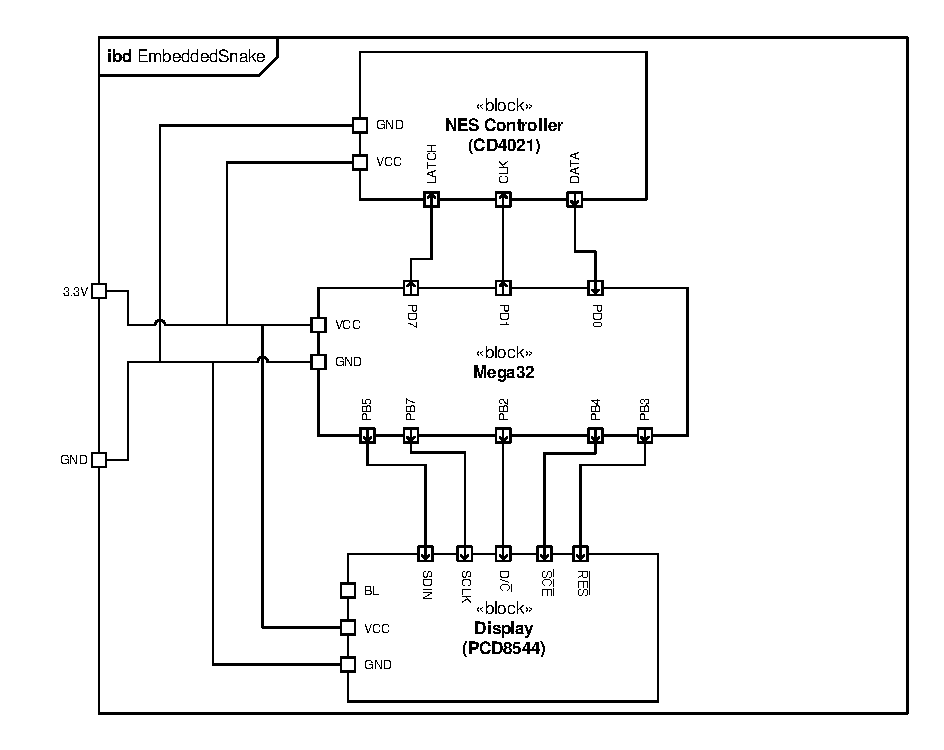
\includegraphics[width=0.8\textwidth, trim={10mm 5mm 5mm 0mm}, clip]{architecture/ibd}
\caption{Internal Block Diagram}
\label{fig:ibd}
\end{figure}

\chapter{Architecture}

We have defined three blocks that outlines our system, as seen in the Block Definition Diagram in Figure~\ref{fig:bdd}. The official responsibilities of the blocks in Figure~\ref{fig:bdd} is as follows:

\begin{itemize}
	\item \textbf{Mega32}: Runs the game, processes input from the controller and draws game on the display.
	\item \textbf{Display}: Displays the game.
	\item \textbf{Controller}: Controls the game.
\end{itemize}

\begin{figure}
\centering
\includegraphics[width=0.7\textwidth, trim={5mm 5mm 5mm 0mm}, clip]{architecture/bdd}
\caption{Block Definition Diagram}
\label{fig:bdd}
\end{figure}

We've identified the Display as a PCD8544. We've also found out that the NES controller uses a CD/TC4021 (8-stage static shift register) to store the state of the controller. Therefore, we'll have write at least two drivers for our system: one to interface the display and one to interface the controller.

We have chosen to describe our system using an Internal Block Diagram (IBD) as seen in Figure~\ref{fig:ibd}. The IBD shows the connections between the blocks.

\begin{figure}
\centering
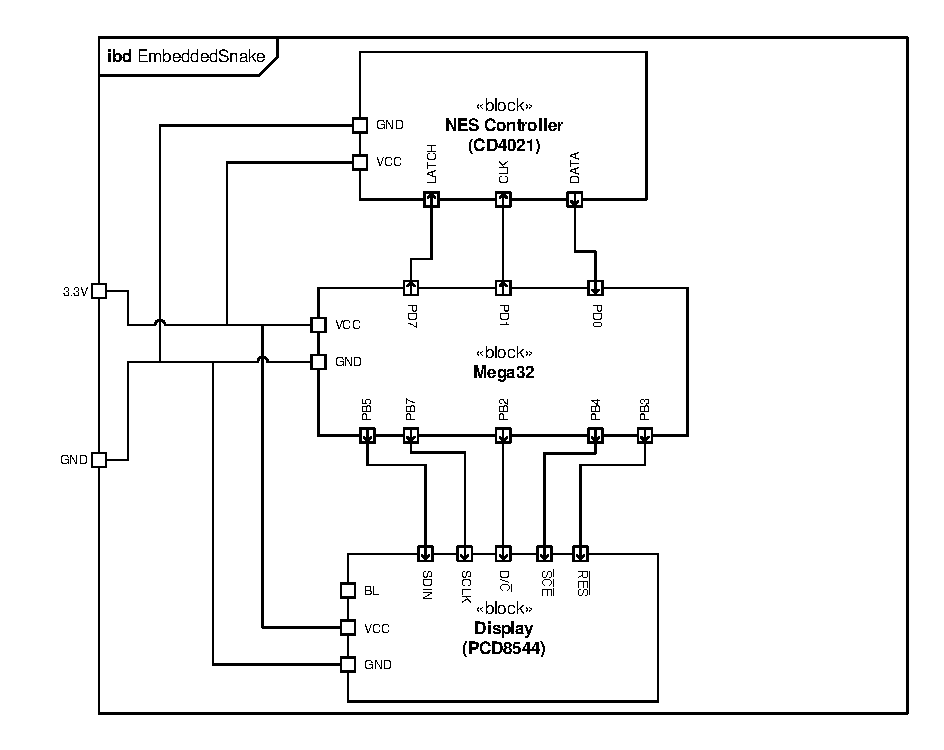
\includegraphics[width=0.8\textwidth, trim={10mm 5mm 5mm 0mm}, clip]{architecture/ibd}
\caption{Internal Block Diagram}
\label{fig:ibd}
\end{figure}

\input{mainmatter/architecture/display/main}
\input{mainmatter/architecture/controller/main}

\chapter{Architecture}

We have defined three blocks that outlines our system, as seen in the Block Definition Diagram in Figure~\ref{fig:bdd}. The official responsibilities of the blocks in Figure~\ref{fig:bdd} is as follows:

\begin{itemize}
	\item \textbf{Mega32}: Runs the game, processes input from the controller and draws game on the display.
	\item \textbf{Display}: Displays the game.
	\item \textbf{Controller}: Controls the game.
\end{itemize}

\begin{figure}
\centering
\includegraphics[width=0.7\textwidth, trim={5mm 5mm 5mm 0mm}, clip]{architecture/bdd}
\caption{Block Definition Diagram}
\label{fig:bdd}
\end{figure}

We've identified the Display as a PCD8544. We've also found out that the NES controller uses a CD/TC4021 (8-stage static shift register) to store the state of the controller. Therefore, we'll have write at least two drivers for our system: one to interface the display and one to interface the controller.

We have chosen to describe our system using an Internal Block Diagram (IBD) as seen in Figure~\ref{fig:ibd}. The IBD shows the connections between the blocks.

\begin{figure}
\centering
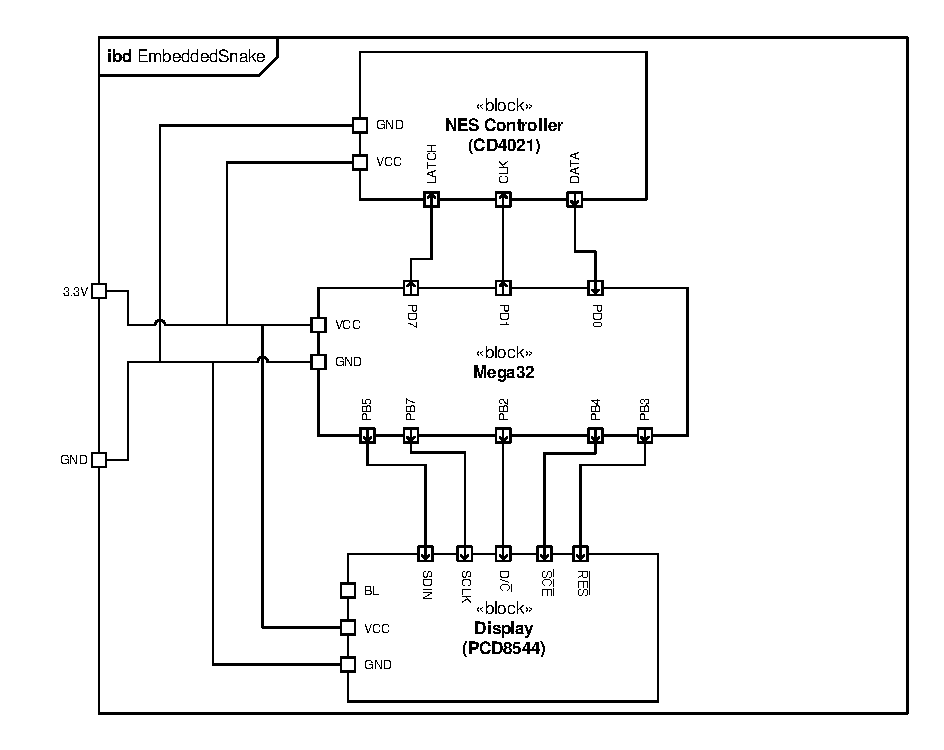
\includegraphics[width=0.8\textwidth, trim={10mm 5mm 5mm 0mm}, clip]{architecture/ibd}
\caption{Internal Block Diagram}
\label{fig:ibd}
\end{figure}

\input{mainmatter/architecture/display/main}
\input{mainmatter/architecture/controller/main}


\chapter{Architecture}

We have defined three blocks that outlines our system, as seen in the Block Definition Diagram in Figure~\ref{fig:bdd}. The official responsibilities of the blocks in Figure~\ref{fig:bdd} is as follows:

\begin{itemize}
	\item \textbf{Mega32}: Runs the game, processes input from the controller and draws game on the display.
	\item \textbf{Display}: Displays the game.
	\item \textbf{Controller}: Controls the game.
\end{itemize}

\begin{figure}
\centering
\includegraphics[width=0.7\textwidth, trim={5mm 5mm 5mm 0mm}, clip]{architecture/bdd}
\caption{Block Definition Diagram}
\label{fig:bdd}
\end{figure}

We've identified the Display as a PCD8544. We've also found out that the NES controller uses a CD/TC4021 (8-stage static shift register) to store the state of the controller. Therefore, we'll have write at least two drivers for our system: one to interface the display and one to interface the controller.

We have chosen to describe our system using an Internal Block Diagram (IBD) as seen in Figure~\ref{fig:ibd}. The IBD shows the connections between the blocks.

\begin{figure}
\centering
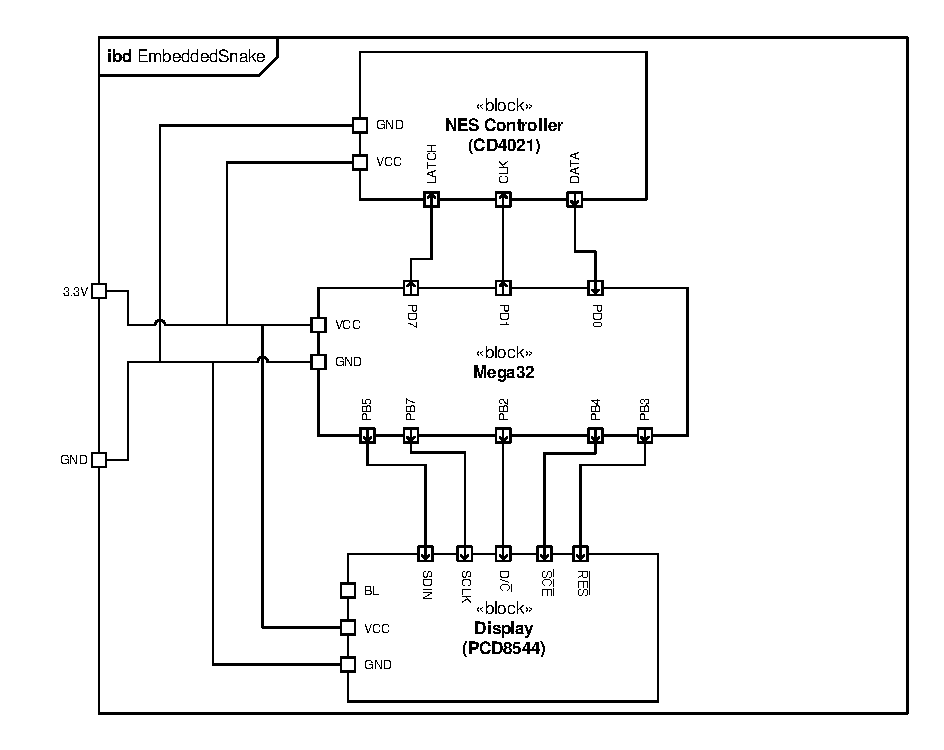
\includegraphics[width=0.8\textwidth, trim={10mm 5mm 5mm 0mm}, clip]{architecture/ibd}
\caption{Internal Block Diagram}
\label{fig:ibd}
\end{figure}

\chapter{Architecture}

We have defined three blocks that outlines our system, as seen in the Block Definition Diagram in Figure~\ref{fig:bdd}. The official responsibilities of the blocks in Figure~\ref{fig:bdd} is as follows:

\begin{itemize}
	\item \textbf{Mega32}: Runs the game, processes input from the controller and draws game on the display.
	\item \textbf{Display}: Displays the game.
	\item \textbf{Controller}: Controls the game.
\end{itemize}

\begin{figure}
\centering
\includegraphics[width=0.7\textwidth, trim={5mm 5mm 5mm 0mm}, clip]{architecture/bdd}
\caption{Block Definition Diagram}
\label{fig:bdd}
\end{figure}

We've identified the Display as a PCD8544. We've also found out that the NES controller uses a CD/TC4021 (8-stage static shift register) to store the state of the controller. Therefore, we'll have write at least two drivers for our system: one to interface the display and one to interface the controller.

We have chosen to describe our system using an Internal Block Diagram (IBD) as seen in Figure~\ref{fig:ibd}. The IBD shows the connections between the blocks.

\begin{figure}
\centering
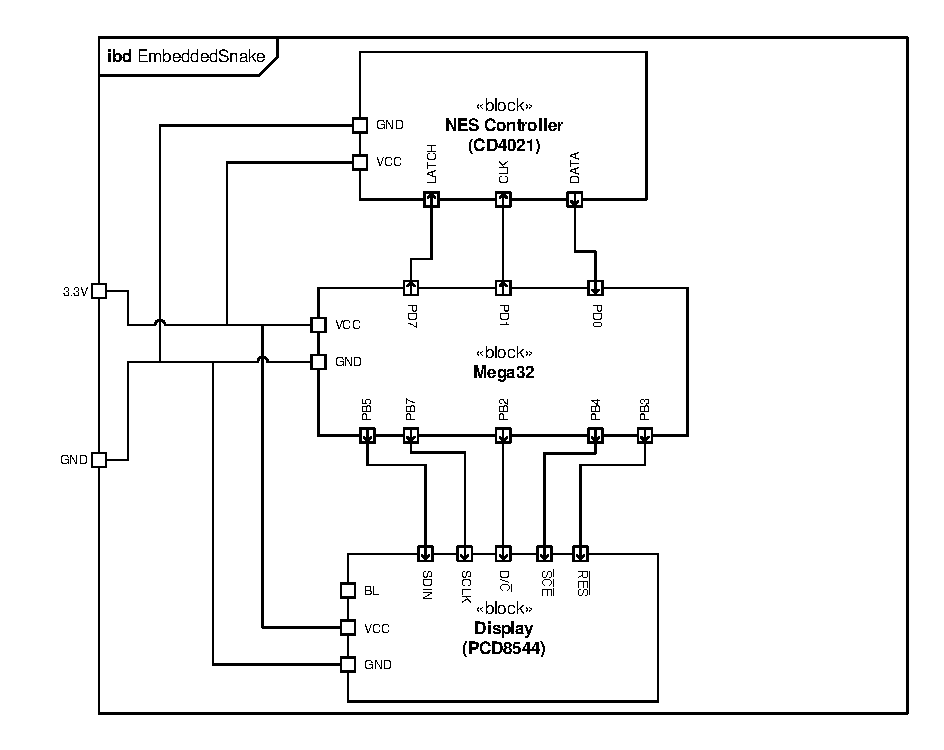
\includegraphics[width=0.8\textwidth, trim={10mm 5mm 5mm 0mm}, clip]{architecture/ibd}
\caption{Internal Block Diagram}
\label{fig:ibd}
\end{figure}

\input{mainmatter/architecture/display/main}
\input{mainmatter/architecture/controller/main}

\chapter{Architecture}

We have defined three blocks that outlines our system, as seen in the Block Definition Diagram in Figure~\ref{fig:bdd}. The official responsibilities of the blocks in Figure~\ref{fig:bdd} is as follows:

\begin{itemize}
	\item \textbf{Mega32}: Runs the game, processes input from the controller and draws game on the display.
	\item \textbf{Display}: Displays the game.
	\item \textbf{Controller}: Controls the game.
\end{itemize}

\begin{figure}
\centering
\includegraphics[width=0.7\textwidth, trim={5mm 5mm 5mm 0mm}, clip]{architecture/bdd}
\caption{Block Definition Diagram}
\label{fig:bdd}
\end{figure}

We've identified the Display as a PCD8544. We've also found out that the NES controller uses a CD/TC4021 (8-stage static shift register) to store the state of the controller. Therefore, we'll have write at least two drivers for our system: one to interface the display and one to interface the controller.

We have chosen to describe our system using an Internal Block Diagram (IBD) as seen in Figure~\ref{fig:ibd}. The IBD shows the connections between the blocks.

\begin{figure}
\centering
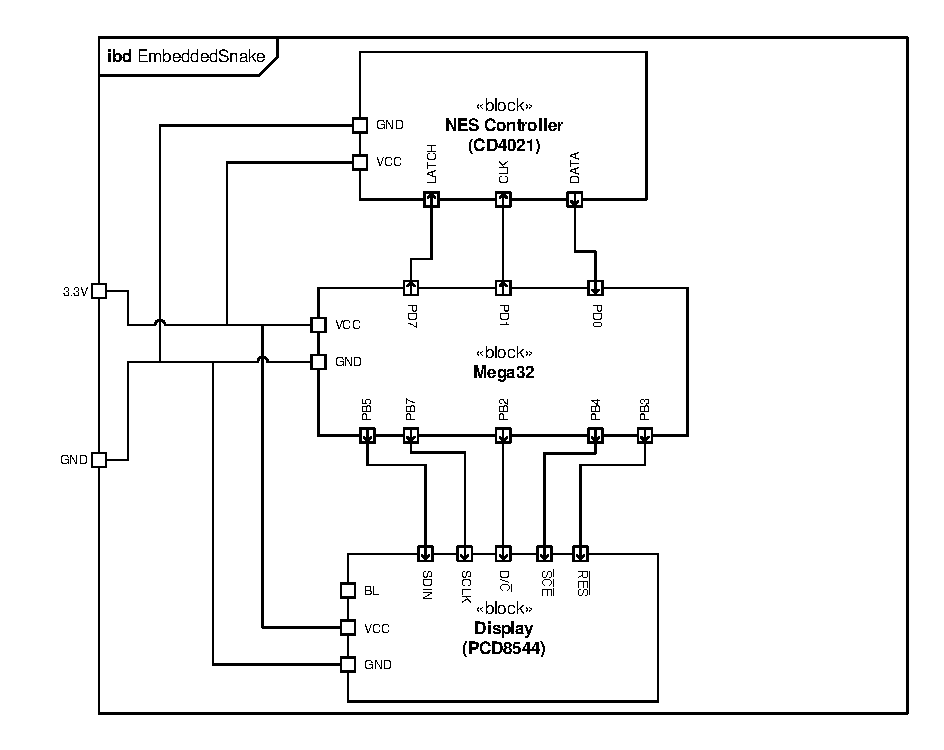
\includegraphics[width=0.8\textwidth, trim={10mm 5mm 5mm 0mm}, clip]{architecture/ibd}
\caption{Internal Block Diagram}
\label{fig:ibd}
\end{figure}

\input{mainmatter/architecture/display/main}
\input{mainmatter/architecture/controller/main}




% Project overview (system description).
% System description (block diagrams and figures are desirable).
